\chapter{Optics of a Blurred Object}
\label{Appendix: Blurred Object}

When an imaged object is blurred, its features do not converge to a single distinct point but are instead smeared around an area called circle of confusion. Figure \ref{fig: Blurred object geometry} shows an object of height $H'$ and how light travels from the highest point of the object to interact with the convergent lens in the sketch. The image also shows an object in focus with height $H$ and its image height $h$. Notice how the light rays from the in-focus object make a triangle with its image, it's this geometry that allows for the derivation of relationship between distances $d_f, f $ and $Z$ called thin lens equation, described in equation \ref{equation: Thin Lens equation}. For an out-of-focus object, the relationship between object distance $m$, image distance $Z$ and $f$ is no longer described through the thin lens equation as the geometry of the system has changed. Nevertheless, It is possible to use this new geometry to define new concepts, such as the blurred object magnification $M_{obj}$, which corresponds to the ratio between the size of the out-of-focus object and the image of the in-focus object that shares the light ray that crosses the middle of the lens with the out-of-focus object.

\begin{figure}[htbp]
    \centering
    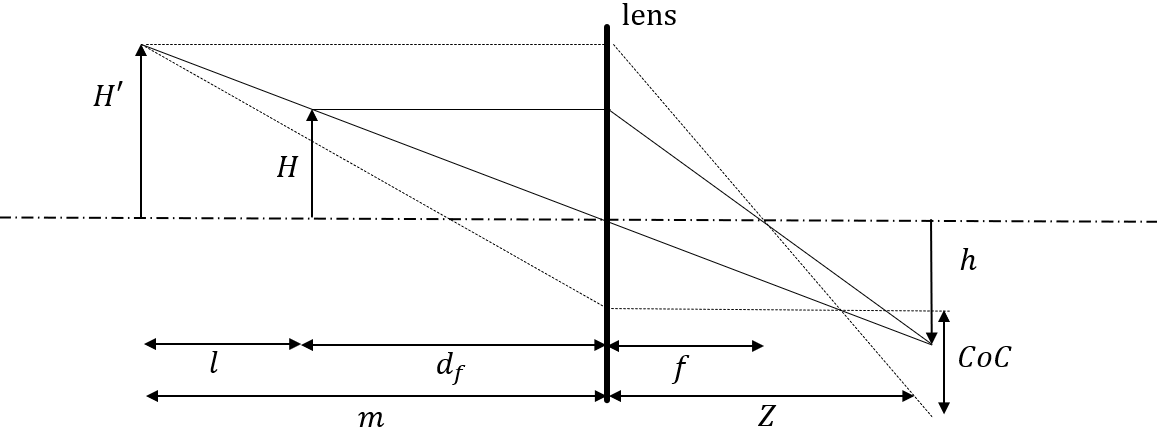
\includegraphics[width=0.8\textwidth]{figures/Blurred Object geometry.png}
    \caption{Geometry of an out of focus object}
    \label{fig: Blurred object geometry}
\end{figure}


\begin{equation}
    \label{equation: Mobj definition}
    M_{obj} = \frac{h}{H'} = \frac{Z}{m}
\end{equation}

This magnification can also be written in terms of the focal length and the in-focus magnification:

\begin{equation}
    \label{equation: Mobj in f and M}
    M_{obj} = \frac{f(1+M)}{m}
\end{equation}

Equivalently to how $M$ can be used to transfer a length from the image plane to the object plane and vice-versa by dividing or multiplying it by $M$, respectively. The same can be done with $M_{obj}$. This way, it is possible to transfer the $CoC$ from the image plane to the blurred object plane. In this same way, $L_{FoV_{obj}}$ was derived in equation \ref{equation: LFoVobj BOS}.

\begin{equation}
    \label{equation: CoCobj transfer}
    CoC_{obj} = \frac{CoC}{M_{obj}}
\end{equation}

By combining equations \ref{equation: CoC in M and S}, \ref{equation: Mobj in f and M} and \ref{equation: CoCobj transfer}, it is possible to obtain:

\begin{equation}
    \label{equation: CoCobj compact}
    CoC_{obj} = \frac{lM}{f_\#(1+M)}
\end{equation}

and rearranging equations \ref{equation: CoCobj transfer} and \ref{equation: Mobj definition}, following the geometry of Figure \ref{fig: Geometry BOS}:

\begin{equation}
    \label{equation: CoCobj expanded}
    CoC_{obj} = \frac{CoC}{M} \frac{m}{d_f} = \frac{CoC}{M} \left( 1 - \frac{l}{m+l}\right)
\end{equation}

Given the spatial resolution $\delta_t$ derived by Gojani \& Obayashi, described by equation 10 on their article \cite{Gojani&Obayashi}.

\begin{equation}
\label{equation: Gojani SR formulation}
    \delta_t = \frac{lM}{f_\#(1+M)} + \frac{\Delta_t}{M} \left( 1 - \frac{l}{m+l}\right)
\end{equation}

If $\Delta_t$ corresponds to the $CoC$ as it is mentioned in Gojani's paper, his blurred circle becomes $\delta_t = 2 \cdot CoC_{obj}$ through equations \ref{equation: CoCobj compact} and \ref{equation: CoCobj expanded}. It is thus proven that Gojani’s formulation predicts a blur circle twice the size of the one established experimentally by Schwarz and Braukmann \cite{Gojani&Obayashi, Schwarz&Braukmann}.
